\documentclass[report, 12pt]{uftreport}

\title{Laboratório 1 -- Minimização Lógica e Hazards}

\author{Pedro Lucas}{Moreira}

\advisor{Prof.}{Tiago}{Almeida}{}

\department{CC}
\class{Linguagens de Descrição de Hardware -- 2026/2}

\date{26}{8}{2026}

\keyword{VHDL}
\keyword{Minimização Lógica}
\keyword{Mapa de Karnaugh}
\keyword{Hazards}

\begin{document}

\frontmatter
\maketitle
\makefrontpage

\mainmatter
\ChapterStart{first}{Questão 1 -- Minimização Lógica}

\chapter{Questão 1 -- Minimização Lógica}

\section{Expressão original}

A função foi obtida a partir do mapa de Karnaugh de 5 variáveis (Figura~\ref{fig:kmap}):

\[
  F(A,B,C,D,E) = \sum m(0,2,5,8,13,18,21,24,29,31)
\]

\section{Minimização por mapa de Karnaugh}

\begin{figure}[htb]
  \centering
  \includegraphics[width=0.6\textwidth]{../01/Screenshot_2026-08-26_21-44-35.png}
  \caption{Mapa de Karnaugh de 5 variáveis (tabelas $A=0$ e $A=1$).}
  \label{fig:kmap}
\end{figure}

Agrupando os 1's do mapa, obtém-se a expressão minimizada:

\[
  F = ABCE + \overline{B}\,\overline{C}\,D\overline{E} + B\overline{C}\,\overline{D}\,\overline{E} + C\overline{D}E + \overline{A}\,\overline{B}\,\overline{C}\,\overline{E}
\]

Em notação de linha (usada no restante do documento e no código-fonte):

\[
  F = ABCE + B'C'DE' + BC'D'E' + CD'E + A'B'C'E'
\]

\section{Tabela verdade}
  \begin{table}[htb]
  \centering
  \caption{Tabela verdade completa (32 combinações).}
  \label{tab:tabela-verdade}
  \begin{tabular}{ccccc|c}
    \toprule
    A & B & C & D & E & F \\
    \midrule
    0 & 0 & 0 & 0 & 0 & 1 \\
    0 & 0 & 0 & 0 & 1 & 0 \\
    0 & 0 & 0 & 1 & 0 & 1 \\
    0 & 0 & 0 & 1 & 1 & 0 \\
    0 & 0 & 1 & 0 & 0 & 0 \\
    0 & 0 & 1 & 0 & 1 & 1 \\
    0 & 0 & 1 & 1 & 0 & 0 \\
    0 & 0 & 1 & 1 & 1 & 0 \\
    0 & 1 & 0 & 0 & 0 & 1 \\
    0 & 1 & 0 & 0 & 1 & 0 \\
    0 & 1 & 0 & 1 & 0 & 0 \\
    0 & 1 & 0 & 1 & 1 & 0 \\
    0 & 1 & 1 & 0 & 0 & 0 \\
    0 & 1 & 1 & 0 & 1 & 1 \\
    0 & 1 & 1 & 1 & 0 & 0 \\
    0 & 1 & 1 & 1 & 1 & 0 \\
    1 & 0 & 0 & 0 & 0 & 0 \\
    1 & 0 & 0 & 0 & 1 & 0 \\
    1 & 0 & 0 & 1 & 0 & 1 \\
    1 & 0 & 0 & 1 & 1 & 0 \\
    1 & 0 & 1 & 0 & 0 & 0 \\
    1 & 0 & 1 & 0 & 1 & 1 \\
    1 & 0 & 1 & 1 & 0 & 0 \\
    1 & 0 & 1 & 1 & 1 & 0 \\
    1 & 1 & 0 & 0 & 0 & 1 \\
    1 & 1 & 0 & 0 & 1 & 0 \\
    1 & 1 & 0 & 1 & 0 & 0 \\
    1 & 1 & 0 & 1 & 1 & 0 \\
    1 & 1 & 1 & 0 & 0 & 0 \\
    1 & 1 & 1 & 0 & 1 & 1 \\
    1 & 1 & 1 & 1 & 0 & 0 \\
    1 & 1 & 1 & 1 & 1 & 1 \\
    \bottomrule
  \end{tabular}
\end{table}

\section{Diagrama lógico}

\begin{figure}[htb]
  \centering
  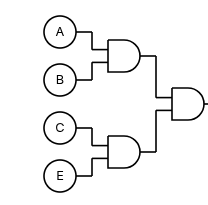
\includegraphics[width=0.6\textwidth]{../01/diagramalogico.png}
\end{figure}

\section{Implementação VHDL estrutural (sem minimização)}

\begin{lstlisting}[language=VHDL, caption={Circuito implementado como OR dos mintermos (e.vhd).}, label={lst:and-gate}]
library ieee;
use ieee.std_logic_1164.all;

entity and_gate is
    port (
        A   : in  std_logic;
        B   : in  std_logic;
        C   : in std_logic;
        D   : in std_logic;
        E   : in std_logic;

        F   : out std_logic
    );
end entity and_gate;

architecture rtl of and_gate is
begin
    F <= (not A and not B and not C and not D and not E)
        or (not A and not B and not C and D and not E)
        or (not A and not B and C and not D and E)
        or (not A and B and not C and not D and not E)
        or (not A and B and C and not D and E)
        or (A and not B and not C and D and not E)
        or (A and not B and C and not D and E)
        or (A and B and not C and not D and not E)
        or (A and B and C and not D and E)
        or (A and B and C and D and E);
end architecture rtl;
\end{lstlisting}

\section{Simulação no Quartus}

\begin{lstlisting}[language=VHDL, label={lst:tb-and-gate}]
library ieee;
use ieee.std_logic_1164.all;
use ieee.numeric_std.all;

entity tb_and_gate is
end entity tb_and_gate;

architecture sim of tb_and_gate is
    signal A, B, C, D, E, F : std_logic;
begin
    uut: entity work.and_gate
        port map (
            A => A,
            B => B,
            C => C,
            D => D,
            E => E,
            F => F
        );

    stim: process
        variable v : std_logic_vector(4 downto 0);
    begin
        for i in 0 to 31 loop
            v := std_logic_vector(to_unsigned(i, 5));
            A <= v(4);
            B <= v(3);
            C <= v(2);
            D <= v(1);
            E <= v(0);
            wait for 10 ns;
        end loop;
        wait;
    end process;
end architecture sim;
\end{lstlisting}

\begin{figure}[htb]
  \centering
  \includegraphics[width=0.9\textwidth]{../01/image.png}
\end{figure}

\section{Teste na DE1}

\begin{lstlisting}[language=VHDL, label={lst:and-gate}]
library ieee;
use ieee.std_logic_1164.all;

entity and_gate is
    port (
        SW0   : in  std_logic;
        SW1   : in  std_logic;
        SW2   : in  std_logic;
        SW3   : in  std_logic;
        SW4   : in  std_logic;

        LEDR1 : out std_logic
    );


end entity and_gate;

architecture rtl of and_gate is
begin
    LEDR1 <= (not SW0 and not SW1 and not SW2 and not SW3 and not SW4)
        or (not SW0 and not SW1 and not SW2 and SW3 and not SW4)
        or (not SW0 and not SW1 and SW2 and not SW3 and SW4)
        or (not SW0 and SW1 and not SW2 and not SW3 and not SW4)
        or (not SW0 and SW1 and SW2 and not SW3 and SW4)
        or (SW0 and not SW1 and not SW2 and SW3 and not SW4)
        or (SW0 and not SW1 and SW2 and not SW3 and SW4)
        or (SW0 and SW1 and not SW2 and not SW3 and not SW4)
        or (SW0 and SW1 and SW2 and not SW3 and SW4)
        or (SW0 and SW1 and SW2 and SW3 and SW4);
end architecture rtl;

\end{lstlisting}

\chapter{Questão 2 -- Hazards}

\section{Implementação na DE1}

\begin{lstlisting}[language=VHDL, label={lst:and-gate}]
library ieee;
use ieee.std_logic_1164.all;

entity and_gate is
    port (
        A   : in  std_logic;
        B   : in  std_logic;
        C   : in std_logic;

        Y  : out std_logic
    );
end entity and_gate;

architecture rtl of and_gate is
begin

    Y <= (A and B) or (not B and C);

end architecture rtl;
\end{lstlisting}


\section{Simulação funcional}

\begin{figure}[htb]
  \centering
  \includegraphics[width=0.9\textwidth]{../02/image.png}
\end{figure}

\section{Simulação de timing}

\section{Explicação do hazard}

O circuito implementa $Y = A \cdot B + \overline{B} \cdot C$. O sinal $B$ aparece nos dois termos da soma, direto em um, invertido no outro, e cada caminho passa por um número diferente de portas até chegar ao OR final (um deles atravessa um inversor extra). Isso gera um atraso de propagação desigual entre os dois termos.

A correção padrão é adicionar o termo de consenso redundante à expressão:

$$Y = A \cdot B + \overline{B} \cdot C + A \cdot C$$

Esse termo mantém a saída em $1$ durante a transição de $B$ sempre que $A = C = 1$, cobrindo a lacuna sem alterar a tabela-verdade do circuito.


\backmatter

\end{document}
